\noindent %Agregar siempre que de por culo la indentación
\chapter{Resultados}
%Descripción de los datos obtenidos. No es un análisis de la conclusión, llegará en el capitulo que viene. Es simplemente una ordenación de los datos
\section{Análisis automático}
    A partir del análisis automático descritos en el apartado anterior. Hemos obtenido una proporción entre el dialogo de varones y mujeres. Siendo 0\% exclusivo de los varones y 100\% exclusivo de las mujeres.
    
    \begin{figure}
        \centering
        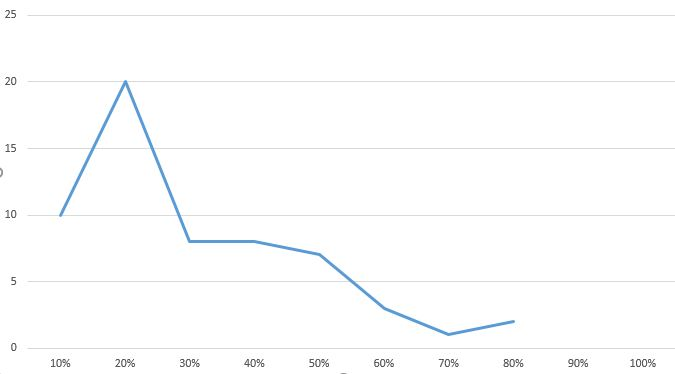
\includegraphics[scale=0.7]{Images/distribucion.jpg}
        \caption{ocurrencias en tramos del 10\% de proporción de diálogo por género}
    \end{figure}
    
\newpage
\section{Análisis manual}
    A partir del análisis manual hemos realizado preguntas diferentes, debido a la diferencia de las pruebas que hemos podido automatizar y las que no. Nuestra intención ha sido la de automatizar lo mas posible para poder abarcar el total de las películas de Disney y eventualmente poder mejorar la calidad de los datos. Pero nos hemos encontrado con diferentes fuentes y formatos para los mismos datos de cada película. Especialmente debido a la naturaleza intelectual de los datos y en menor medida debido a la falta de interés de normalizar estos parámetros. En el siguiente gráfico vemos una serie de películas ordenadas temporalmente con la tasa de tiempo de hombres y mujeres sin apreciarse especial inclinación a un lado u otro. Igualmente, en la suma total de tiempos se ve una desviación de la mitad, fácilmente atribuible al ruido.
    \begin{figure}
        \centering
        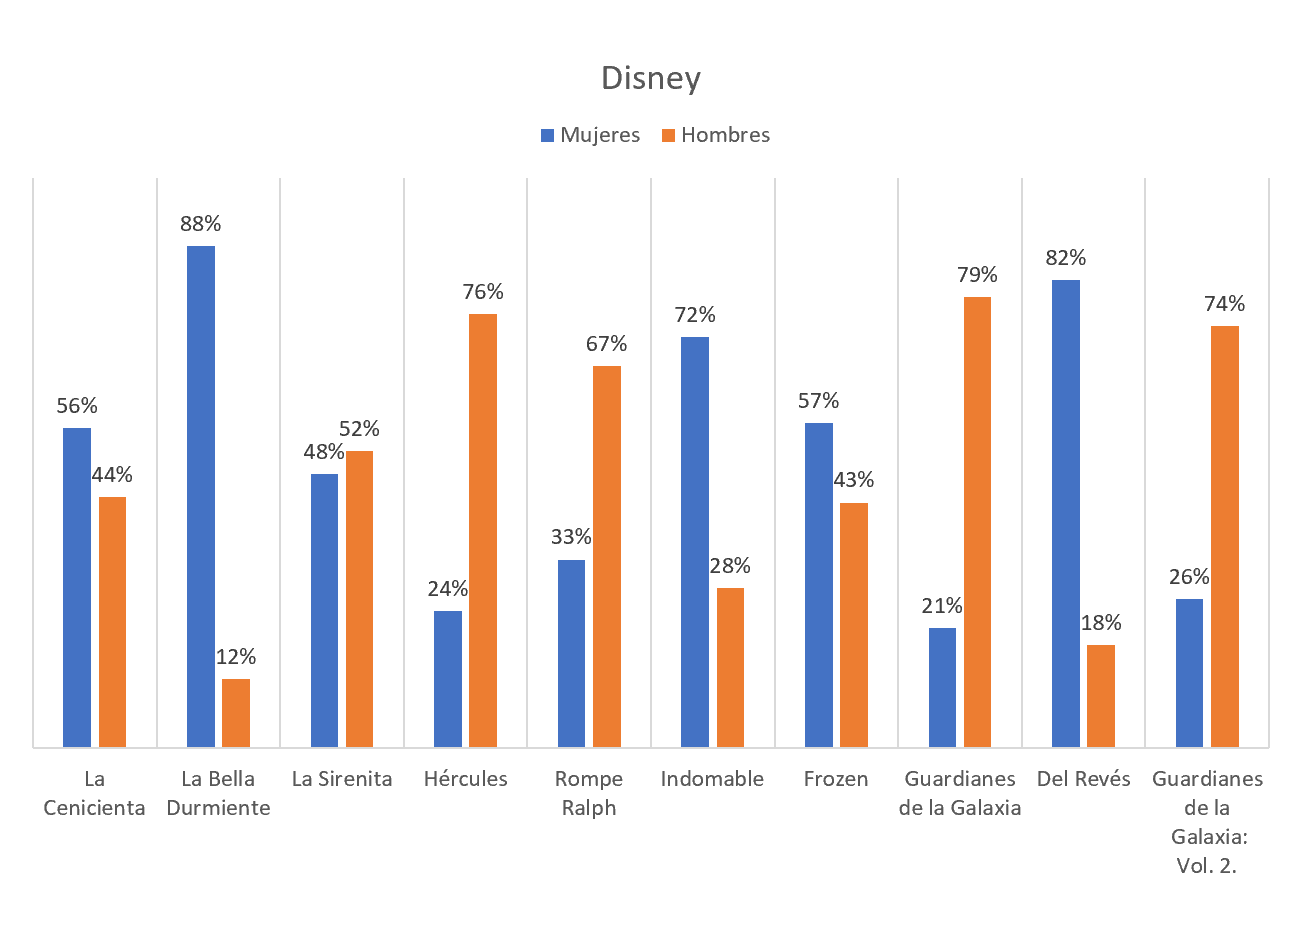
\includegraphics[scale=0.7]{Images/peliculas.png}
        \caption{Distribución de las líneas de diálogo por sexos y películas ordenadas por fecha de estreno}
    \end{figure}
    \begin{figure}
        \centering
        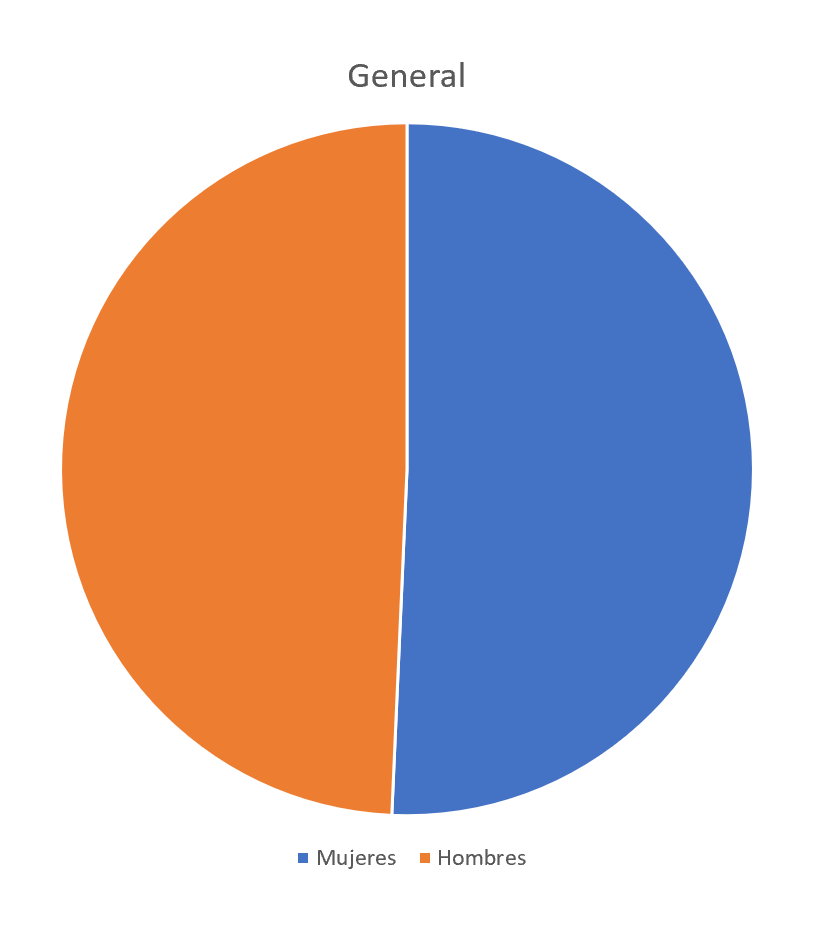
\includegraphics[scale=0.7]{Images/general.png}
        \caption{Distribución de las líneas de diálogo por sexos dentro de las películas analizadas}
    \end{figure}